\tikzstyle{vertex}=[auto=left,circle,fill=black!25,minimum size=20pt,inner sep=0pt]
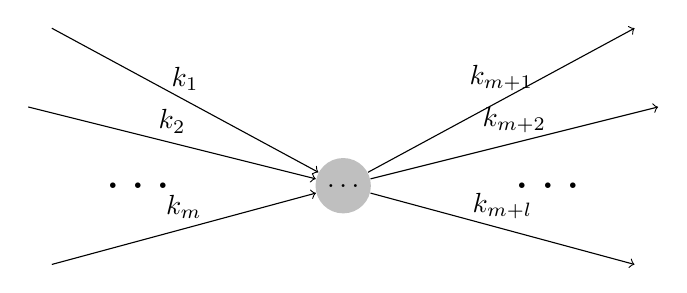
\begin{tikzpicture}
	
	\node[vertex] (sc) at (4,0) {$\dots$};
	
	\draw[->] (0.3,2)--(sc) node [midway, above] {$k_1$};
	\draw[->] (0,1)--(sc) node [midway, above] {$k_2$};
	\draw[->] (0.3,-1)--(sc) node [midway, above] {$k_m$};
	
	\path (1.4,0.6) -- (1.4,-0.6)  node [font=\huge,midway]{$\dots$};
	
	
	\draw[->] (sc)--(8-0.3,2) node [midway, above] {$k_{m+1}$};
	\draw[->] (sc)--(8,1) node [midway, above] {$k_{m+2}$};
	\draw[->] (sc)--(8-0.3,-1) node [midway, above] {$k_{m+l}$};
	
	\path (6.6,0.6) -- (6.6,-0.6)  node [font=\huge, midway]{$\dots$};
\end{tikzpicture}

В классической нормировке вероятность соударения $k_1 ... k_m \leftarrow k_{m+1} ... k_{m+l}$ равна квадрату S-матрицы.
\begin{equation*}
	P = | \mel{k_1 ... k_m}{S}{k_{m+1} ... k_{m+l}}|^2
\end{equation*}

Состояния в классическом и релятивистком случае нормируются так:
\begin{align*}
	\bra{k}\ket{p} = \delta_{kp}\\
	\bra{k}\ket{p} = 2E_k (2\pi)^3 \delta^{(3)}(\vec{k}-\vec{p} \,)
\end{align*}

Тогда классический вектор выражается через релятивисткий, (полагая, что $(2\pi)^3 \delta^{(3)}(0) = V$ --- объем пространства).

\begin{equation*}
	\ket{p}_K =\cfrac{ \ket{p}_R}{\sqrt{2EV}}
\end{equation*}

а вероятность столкновения

\begin{equation*}
	P = VT \prod_{i} \cfrac{1}{2 E_i V} \cdot |\mathcal{M}|^2 (2\pi)^4 
	\delta^{(4)}(k_{out} - k_{in})
\end{equation*}

В этом выражении $T$ --- это интервал времени, т.е. $dt$, а $V$ --- объем, т.е. $d^3\vec{x}$.

Суммирование по импульсам в классическом случае --- это интеграл с дифференциалом
\[
	\cfrac{Vd^3\vec{k}}{(2\pi)^3}
\]

При этом у входных импульсов есть еще функция распределения

В итоге, интеграл столкновений выглядит следующим образом

\begin{equation*}
	\frac{dN}{dt} = \frac{P}{T} = \int d^3\vec{r} \prod_{i} \cfrac{d^3\vec{k}_i}{2 E_i (2\pi)^3} |\mathcal{M}|^2 (2\pi)^4 \delta^{(4)}(k_{out} - k_{in}) \prod_{in} f_B(\vec{r},\vec{k}_i)
\end{equation*}

Все входные интегралы умножаются на функцию распределения, которая в Больцмановском случае равна

\begin{equation*}
	f_B(\vec{r},\vec{k}) = \cfrac{n}{(2\pi mT)^{3/2}} \, \exp(-\frac{\vec{k}^2}{2mT})
\end{equation*}



